\chapter{Análise dos Conjuntos de \textit{Benchmark}}\label{ch:analise}

Neste capítulo as métricas apresentadas no Capítulo~\ref{ch:medidas} são 
utilizadas para analisar as instâncias de \textit{benchmark} descritas no
Capítulo~\ref{ch:instancias}. 
Esta análise tem como objetivo avaliar a dispersão dos valores de dinamismo e 
urgência das instâncias de cada conjunto de \textit{benchmark} e com isso 
permitir que futuras pesquisas possam se basear nos
dados expostos nesse capítulo para escolher conjuntos de \textit{benchmark} que
representem cenários de interesse prático para teste.






\section{Distribuição do grau de dinamismo e da urgência}

Cada um dos gráficos apresentados na 
Figura~\ref{fig:scatterplot_instance_planing_horizon} representa um conjunto 
de instâncias de \textit{benchmark} diferente. 
Cada ponto no gráfico corresponde aos valores de urgência média normalizada 
(eixo vertical) e dinamismo (eixo horizontal) de uma das instâncias desse 
conjunto.
A normalização da urgência média é feita de maneira que o valor zero represente
uma urgência média igual a zero e o valor um represente a maior urgência média
encontrada dentro do conjunto de instâncias de \textit{benchmark} em questão.
A figura mostra o acúmulo dos pontos, o que demonstra a falta
de diversidade entre instâncias de um mesmo conjunto de \textit{benchmark},
para os critérios considerados.

% TODO Rodrigo: porque o que está relatado no parágrafo anterior é ruim?

A Figura~\ref{fig:dynamism_boxplot_planing_horizon} mostra os mesmos valores de
dinamismo exibidos na Figura~\ref{fig:scatterplot_instance_planing_horizon}, 
entretanto em forma de diagrama de caixas, em que 50\% dos valores de dinamismo
de cada conjunto de \textit{benchmark} estão contidos nas caixas.
A mediana dos valores é demarcada por um risco vertical dentro desta caixa e os
limites inferiores ($LI$) e superiores ($LS$) são demarcados pelos segmentos 
de reta vertical externos às caixas, cujos valores podem ser calculados 
por:

\begin{equation}
  LI = Q_1 - 1{,}5 \cdot AIQ,
\end{equation}

\begin{equation}
  LS = Q_3 + 1{,}5 \cdot AIQ.
\end{equation}

\begin{equation}
  AIQ = Q_3 - Q_1
\end{equation}

Em que:
\begin{itemize}
  \item $Q_1$: primeiro quartil, correspondendo a 25\% das menores medidas.
  \item $Q_3$: terceiro quartil, correspondendo a 75\% das menores medidas.
  \item $AIQ$: amplitude interquartil.
\end{itemize}

Ainda no gráfico de caixas, podem ser encontrados pequenos losangos, indicando
valores não contidos no intervalo $[LI; LS]$.

Pode-se observar que quatro dos seis conjuntos estudados possuem medianas 
menores que 0,1 e uma alta concentração de instâncias com dinamismo menor que 
0,2, indicando uma falta de diversificação das instâncias desses quatro 
conjuntos. 
Vale destacar que quanto maior o dinamismo, maior a quantidade de vezes que
necessita-se usar o algoritmo de otimização.
Portanto, conjuntos de \textit{benchmark} com baixo valor de dinamismo podem
beneficiar algoritmos que retornem bons resultados a custo de um longo tempo de
computação.

Outro fator interessante a se destacar é a escassez de instâncias com dinamismo
entre 0,45 e 0,6. 
\citeonline{van_lon_measures_2016} afirmam que este intervalo de valores de 
dinamismo ocorre em cenários gerados por distribuições Poisson homogêneas.
Tendo em vista que as chegadas de pedidos de viagem em sistemas de 
\textit{dial-a-ride} acontecem de forma a se assemelhar com uma distribuição de
Poisson homogênea \cite{schilde_metaheuristics_2011}, a falta de instâncias 
com esses valores de dinamismo prejudica a análise de cenários realísticos.

% TODO mudar imagem para .eps
\begin{figure}[H]
    \centering
    \makebox[\textwidth]
    {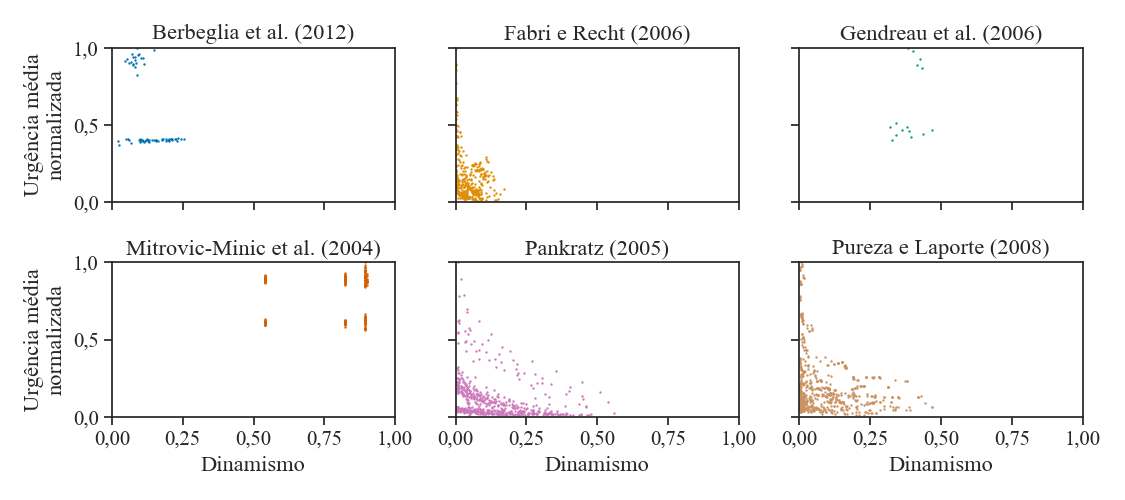
\includegraphics[width=\textwidth]
    {fig/analyses/scatterplot_dynamism_x_urgency_mean_norm_max_planing_horizon.png}}
    \caption{Gráfico de dispersão da urgência média e do dinamismo de cada 
    conjunto de \textit{benchmark}}
    \label{fig:scatterplot_instance_planing_horizon}
\end{figure}

% TODO mudar imagem para .eps
\begin{figure}[H]
    \centering
    \makebox[\textwidth]
    {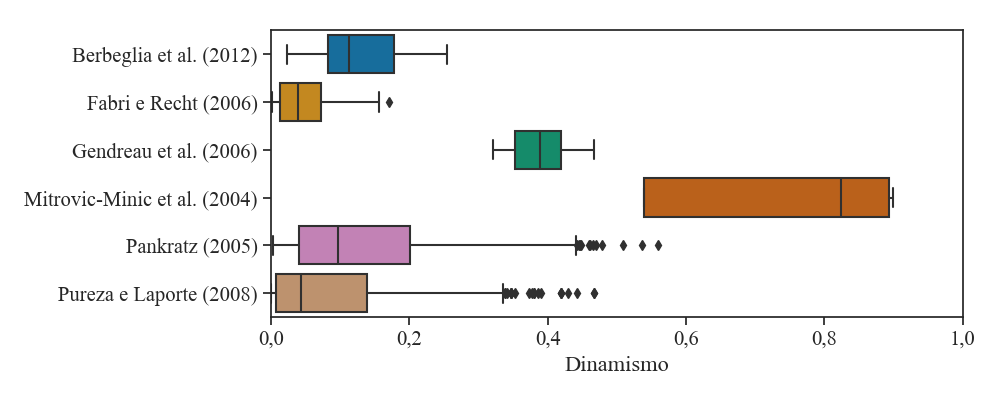
\includegraphics[width=\textwidth]
    {fig/analyses/boxplot_dynamism_by_benchmark_planing_horizon.png}}
    \caption{Diagrama de caixa dos valores de dinamismo por \textit{benchmark}}
    \label{fig:dynamism_boxplot_planing_horizon}
\end{figure}





\section{Correlação entre limites inferiores das janelas de tempo de coleta e
os instantes de chegada dos pedidos}

Pela definição de dinamismo apresentada na Seção~\ref{sec:dinamismo}, os 
intervalos entre os instantes de chegadas dos pedidos são os principais fatores
determinadores do valor de dinamismo de uma instância.
Portanto, para que um conjunto de \textit{benchmark} possua instâncias cujos 
valores de dinamismo sejam distintos entre si, se faz necessário que a 
distribuição dos instantes de chegada seja diferente entre instâncias 
\cite{van_lon_measures_2016}.

Entretanto, no Capítulo~\ref{ch:instancias}, percebe-se que grande parte dos 
conjuntos de \textit{benchmark} apresentados um único método de 
dinamização, não possibilitando a diversificação do tamanho dos intervalos de 
tempo entre instâncias.
A única exceção é o \citeonline{pankratz_benchmark_2009} que varia o valor 
$\maneuverTime$ garantido a geração de instâncias cujos instantes de chegadas 
diferem entre si.
Porém, mesmo variando esse valor, não foi alcança uma variedade muito grande de
dinamismo entre cenários 
(Figuras~\ref{fig:scatterplot_instance_planing_horizon}~e
\ref{fig:dynamism_boxplot_planing_horizon}).

Dentre os métodos de dinamização apresentados no Capítulo~\ref{ch:instancias} é 
comum a utilização dos limites da janela de tempo de coleta para o cálculo dos 
instantes de chegada dos pedidos.
O objetivo do uso deste parâmetro na hora de computar o instante de chegada do 
pedido é garantir que os pedidos possam ser atendidos em tempo hábil.
Entretanto, isso faz com que a distribuição das janelas de tempo das instâncias
estáticas influenciem altamente na distribuição dos instantes de chegadas nos 
pedidos.
Portanto, se a distribuição dos limites das janelas de tempo possuir acúmulo 
de valores, pode-se esperar que os instantes de chegada dos pedidos também  
possua o mesmo acúmulo.

% TODO Rodrigo: pouco visual. Exemplo?

As Figuras~\ref{fig:hist_pickup_lower_tw}~e~\ref{fig:hist_pickup_upper_tw} 
apresentam a distribuição dos limites inferiores e superiores das janelas de 
tempo de coleta de cada um dos conjuntos de \texti{benchmark} normalizados 
pelos horizontes de planejamento de suas respectivas instâncias.
Nota-se que os limites inferiores tendem, em sua maioria, a acumular no início 
do horizonte de planejamento.
Já os limites superiores possuem uma distribuição menos aglutinada, 
porém apresentando ainda pontos de concentração.

% TODO mudar imagem para .eps
\begin{figure}[h]
    \centering
    \makebox[\textwidth]
    {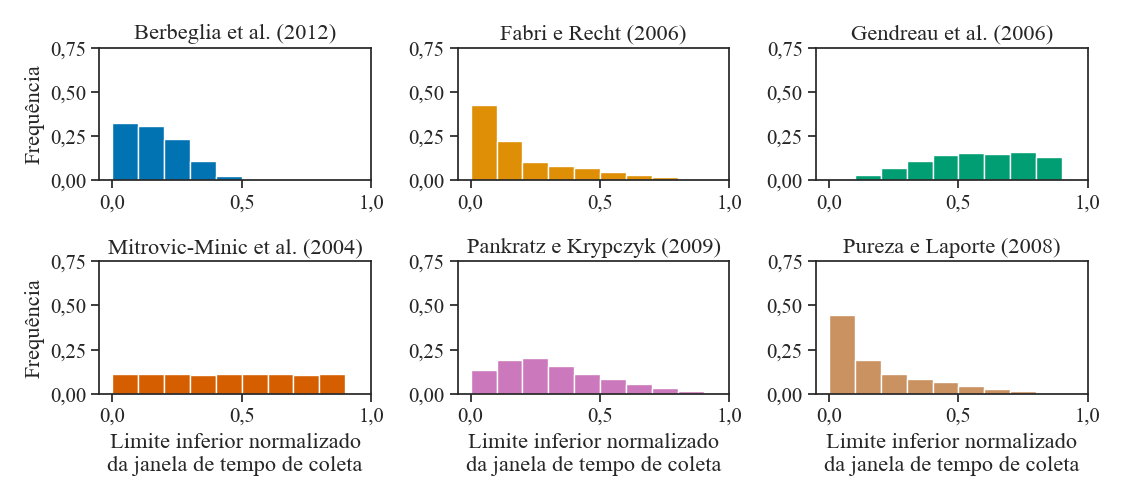
\includegraphics[width=\textwidth]
    {fig/analyses/hist_real_pltw_norm_h_by_benchmark_planing_horizon.png}}
    \caption{Histograma dos limites inferiores das janelas de tempo 
             de coleta por conjunto de \textit{benchmark}}
    \label{fig:hist_pickup_lower_tw}
\end{figure}

% TODO mudar imagem para .eps
\begin{figure}[h]
    \centering
    \makebox[\textwidth]
    {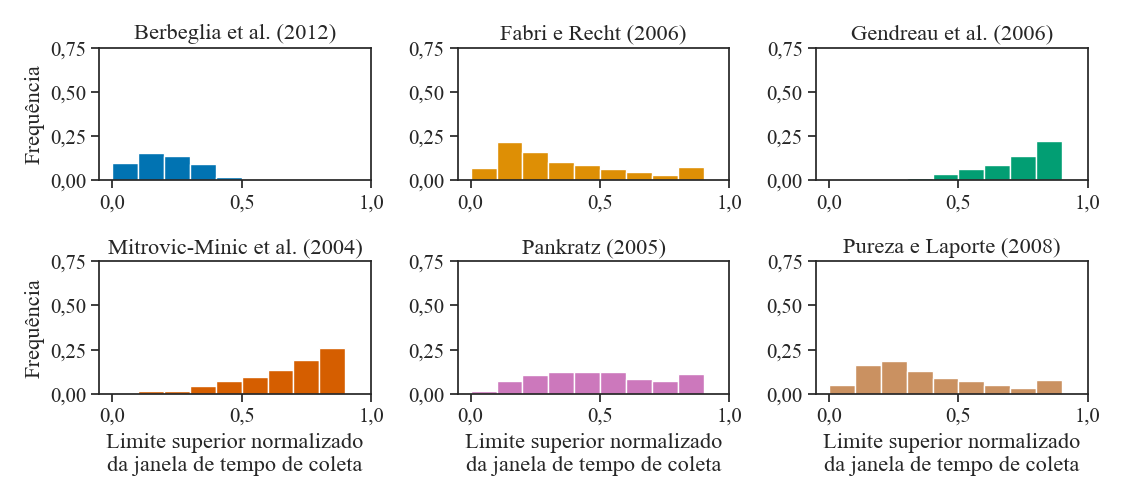
\includegraphics[width=\textwidth]
    {fig/analyses/hist_putw_norm_h_by_benchmark_planing_horizon.png}}
    \caption{Histograma dos limites superiores das janelas de tempo de 
             coleta por conjunto de \textit{benchmark}}
    \label{fig:hist_pickup_upper_tw}
\end{figure}

% TODO Rodrigo: o que tem a ver com as características das instâncias?
% com técnica de dinamização

Como discutido anteriormente, esse acúmulo dos limites da janela de coleta pode
ser propagado para a distribuição dos instantes de chegadas.
Essa propagação pode ser visualizada na Figura~\ref{fig:hist_arrival_time}, que
apresenta as distribuições dos instantes de chegada dos pedidos.
Observa-se que alguns dos acúmulos apresentados nas 
Figuras~\ref{fig:hist_pickup_lower_tw}~e~\ref{fig:hist_pickup_upper_tw} podem 
ser também observados na Figura~\ref{fig:hist_arrival_time}.

% TODO Rodrigo: O que isso quer dizer? Como é feita a propagação?

\begin{figure}[h]
    \centering
    \makebox[\textwidth]
    {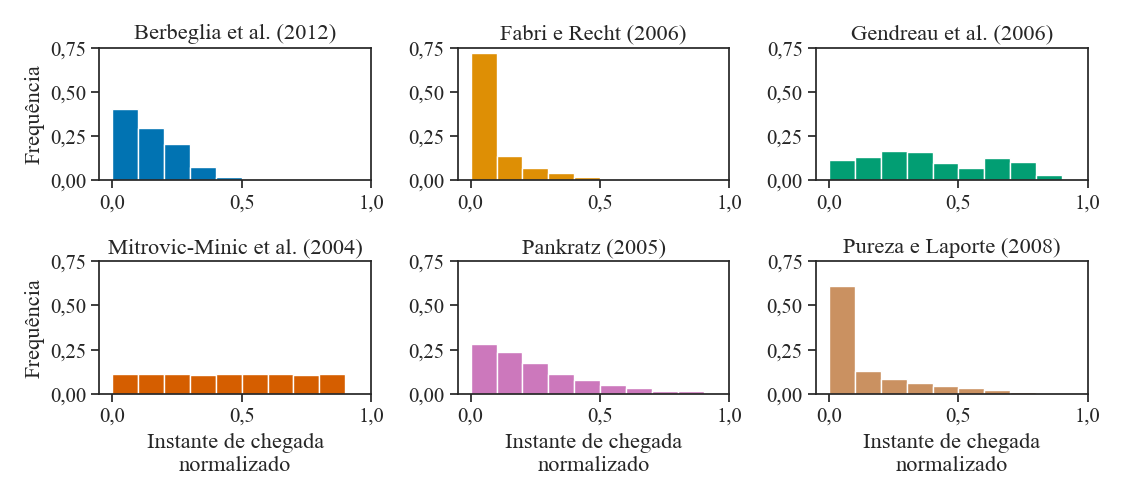
\includegraphics[width=\textwidth]
    {fig/analyses/hist_arrival_time_norm_h_by_benchmark_planing_horizon.png}}
    \caption{Histograma dos instantes de chegada para cada conjunto 
             de \textit{benchmark}}
    \label{fig:hist_arrival_time}
\end{figure}

A Tabela~\ref{tab:correlation_real_pltw_norm_h_and_arrival_time_norm_h} 
apresenta, os valores das correlações entre os instantes de chegada dos 
pedidos e os limites inferiores das janelas de tempo de coleta dos pedidos.
Percebe-se uma correlação alta para as instâncias de 
\citeonline{berbeglia_hybrid_tabu_2012}, 
\citeonline{mitrovic-minic_waiting_2004}, 
\citeonline{pankratz_dynamic_2005} e 
\citeonline{pureza_laporte_waiting_2008}.
Já os conjuntos propostos por \citeonline{fabri_dynamic_2006}  e 
\citeonline{gendreau_neighborhood_2006} possuem uma correlação baixa entre estes 
dois parâmetros, que pode ser explicada pelo uso de variáveis aleatórias de 
distribuição uniforme no processo de dinamização ou criação das instâncias.


\begin{table}[H]
    \footnotesize
    \centering
    \caption{Valores de correlação entre os instantes de chegadas normalizados
             e os limites inferiores normalizados das janelas de tempo de
             coleta}
    \label{tab:correlation_real_pltw_norm_h_and_arrival_time_norm_h}
    \begin{tabular}{lr}
        \toprule
        Conjunto de \textit{benchmark}                  & $r$ \\ 
        \midrule
        \citeonline{berbeglia_hybrid_tabu_2012}         & 0,95 \\
        \citeonline{fabri_dynamic_2006}                 & 0,78 \\
        \citeonline{gendreau_neighborhood_2006}         & 0,73 \\
        \citeonline{mitrovic-minic_waiting_2004}        & 1,00 \\
        \citeonline{pankratz_benchmark_2009}            & 0,81 \\
        \citeonline{pureza_laporte_waiting_2008}        & 0,89 \\ 
        \bottomrule
    \end{tabular}
\end{table}


Destaca-se que estes valores de correlação são relativos a uma relação linear
entre as variáveis em questão. Ou seja, ainda podem existir outras relações não
lineares entre o instante de chegada do pedido e o limite inferior da janela
de tempo de coleta.

As Figuras~\ref{fig:scatterplot_pickup_lower_tw_x_arrival_time}~e
\ref{fig:scatterplot_pickup_upper_tw_x_arrival_time} apresentam, 
de forma visual, as correlações entre os instantes de chegada dos 
pedidos e os limites das janelas de tempo de coleta dos pedidos.
Percebe-se uma correlação alta para as instâncias de 
\citeonline{berbeglia_hybrid_tabu_2012}, 
\citeonline{mitrovic-minic_double-horizon_2004}, 
\citeonline{pankratz_benchmark_2009} e 
\citeonline{pureza_laporte_waiting_2008}.
Já os conjuntos propostos por \citeonline{gendreau_neighborhood_2006} e
\citeonline{fabri_dynamic_2006} possuem uma correlação baixa entre estes 
dois valores, que pode ser explicada pelo uso de variáveis aleatórias de 
distribuição uniforme no processo de dinamização das instâncias.

% TODO Rodrigo: Explicar melhor a última frase do parágrafo anterior

% TODO mudar imagem para .eps
\begin{figure}[h]
    \centering
    \makebox[\textwidth]
    {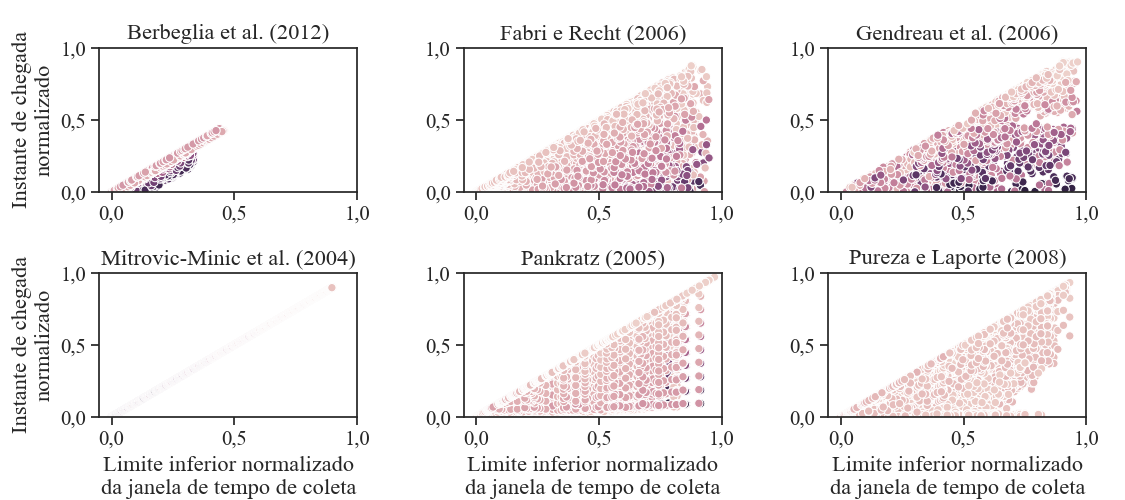
\includegraphics[width=\textwidth]
    {fig/analyses/facetgrid_scatterplot_real_pltw_norm_h_x_arrival_time_norm_h_planing_horizon.png}}
    \caption{Gráfico de dispersão entre o limite inferior da janela de tempo
             de coleta e o instante de chegada do pedido para cada conjunto 
             de \textit{benchmark}}
    \label{fig:scatterplot_pickup_lower_tw_x_arrival_time}
\end{figure}

% TODO mudar imagem para .eps
\begin{figure}[h]
    \centering
    \makebox[\textwidth]
    {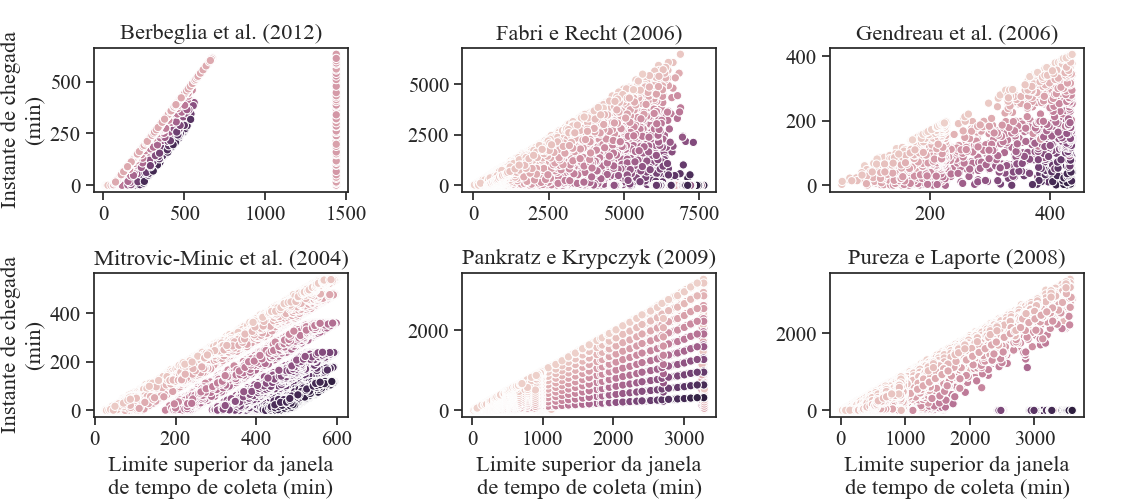
\includegraphics[width=\textwidth]
    {fig/analyses/facetgrid_scatterplot_pickup_upper_tw_x_arrival_time_planing_horizon.png}}
    \caption{Gráfico de dispersão entre o limite superior da janela de tempo 
             de coleta e o instante de chegada do pedido para cada conjunto 
             de \textit{benchmark}}
    \label{fig:scatterplot_pickup_upper_tw_x_arrival_time}
\end{figure}






\section{Presença de pedidos estáticos}

A análise dos valores dos instantes de chegada de cada conjunto mostra que 
nos conjuntos propostos por \citeonline{berbeglia_hybrid_tabu_2012,
fabri_dynamic_2006, pureza_laporte_waiting_2008} uma grande quantidade 
de pedidos chegam no instante zero e, por definição, 
são considerados pedidos estáticos.
A Tabela~\ref{tab:percentage_arrival_time_equal_0} mostra a porcentagem de 
pedidos com instante de chegada igual a zero para cada um dos conjuntos de
\textit{benchmark}.

Acredita-se que este efeito colateral seja também causado pelo uso de métodos de
dinamização baseado nos limites da janela de tempo de entrega e coleta aliado ao
uso de instâncias estáticas que apresentam uma distribuição acumulada destes 
valores, principalmente no início do horizonte de planejamento.
Portanto, ao usar-se os métodos de dinamismo deve-se ter cuidado para que estes
não gerem demasiados pedidos estáticos, o que pode atrapalhar a análise de
algoritmos feitos para atender pedidos dinâmicos.

Destaca-se que esses pedidos estáticos podem também representar
uma condição inicial ao sistema. Mesmo assim, é importante perceber que alguns
métodos de geração de instâncias dinâmicas possuem uma maior probabilidade de
gerar condições iniciais com maior número de pedidos estáticos.

\begin{table}[h]
  \footnotesize
  \centering
  \caption{Porcentagem de pedidos com instante de chegada igual a zero}
  \label{tab:percentage_arrival_time_equal_0}
  \begin{tabular}{lr}
    \toprule
    Conjunto de \textit{benchmark}                  & \% \\
    \midrule
    \citeonline{berbeglia_hybrid_tabu_2012}         & 10,0 \\
    \citeonline{fabri_dynamic_2006}                 & 20,3 \\
    \citeonline{gendreau_neighborhood_2006}         &  0,7 \\
    \citeonline{mitrovic-minic_double-horizon_2004} &  0,3 \\
    \citeonline{pankratz_benchmark_2009}            &  0,0 \\
    \citeonline{pureza_laporte_waiting_2008}        & 19,5 \\ 
    \bottomrule
  \end{tabular}
\end{table}






\iffalse
\subsection{Atrelamento entre grau de dinamismo e urgência}
A urgência é calculada pela diferença entre o limite 
superior da janela de tempo da coleta e o instante de chegada do pedido, em 
muitos dos métodos de dinamização apresentados, é calculado
usando a janela de tempo de coleta como principal parâmetro.
Isso pode acarretar em um atrelamento dos valores de urgência e de dinamismo,
tendo em vista que ambos são gerados a partir da janela de tempo de coleta.
Na \autoref{fig:scatterplot_pickup_lower_tw_x_arrival_time} a coloração dos
pontos indica o valor da urgência de cada pedido, sendo pedidos menos
urgentes representados por tons claros e pedidos mais urgentes por tons
escuros.
Observa-se que nos conjuntos de \textit{benchmark} propostos por
\textcite{berbeglia_hybrid_tabu_2012, 
fabri_dynamic_2006, 
mitrovic-minic_waiting_2004, 
pankratz_dynamic_2005}
a coloração dos pontos varia juntamente com os valores dos eixo vertical 
(instante de chegada do pedido) e dos eixos horizontais (limite inferior da 
janela de tempo de coleta).
Em seu artigo, \textcite{van_lon_measures_2016} afirma que as medidas de
grau de dinamismo e urgência devem ser ortogonais, portanto, uma instância
que possua um grau de dinamismo pode possuir qualquer valor de urgência.
Portanto, os métodos de dinamização estudados possuem uma dificuldade de 
gerar cenários que cubram todo o espectro de possíveis pares de valores entre
dinamismo e urgência.
\fi
